\chapter{Artificial Neural Networks}
\section{Artificial Neuron}
Our brain is composed by biological neurons and an artificial neuron (or AN) is a representation of it. Every AN can gather signals from other nurons or from the environment, and after an elaboration it transmits another signal to all the other ANs that are connected to it \cite{engelbrecht2007computational}. A rapresentation of AN is depicted in \ref{fig:artificial_neuron}. \\
Each connection to the artificial neuron has a numerical weigth associated to it in which the input signal is hold back. The value of the weight can be either positive or negative. In most cases, the sums of each node are weighted and then given as input to a \textit{non-linear} function called \textbf{transfer function} or \textbf{activation function} \cite{artificial_neuron_wiki}. The activate function defines the output value of the node. Typically, the \textit{Step Function}, \textit{Sigmoid Function} and a \textit{Softmax Function} are the most used.

\begin{figure}[!ht]
    \centering
    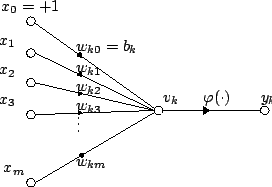
\includegraphics[scale=0.5]{Figures/artificial_neuron.png}
    \caption{Representation of an Artificial Neuron \cite{artificial_neuron_wiki}}
    \label{fig:artificial_neuron}
\end{figure}

\noindent From the mathematical point of view, we can define an artificial neuron as follow: \\
given $m+1$ inputs with signals from $x_1$ to $x_m$ and weights values from $w_0$ to $w_m$. The \textit{bias} is then defined by the input $x_0$ in which a value of 1 will be assigned. The bias value allows us to \textit{shift} the curve of the activation function to a certain direction and it is defined with $w_{k0} = b_k$ \cite{artificial_neuron_wiki}. \\
The output of the AN is:

\begin{equation*}
    y_k = \varphi \left ( \sum_{j=0}^{m} w_{kj} x_j \right )
\end{equation*}

\section{Network Function}
When there are many aritificial neurons interconnected between each other in the different layers, we form a \textit{network}. \ref{fig:ann} shows an example of ANN where the \textbf{inputs} are represented by the first layer in which they send data through the connection to the second group of neuron. The connection between two neuros is called \textit{synapses} where the \textbf{weigth} is stored. The second layer is connected to the third one that represents the \textbf{output} of the network. There can be multiple stratums between the inputs and the outputs and these are called \textit{hidden layers}. \\

\begin{figure}[!ht]
    \centering
    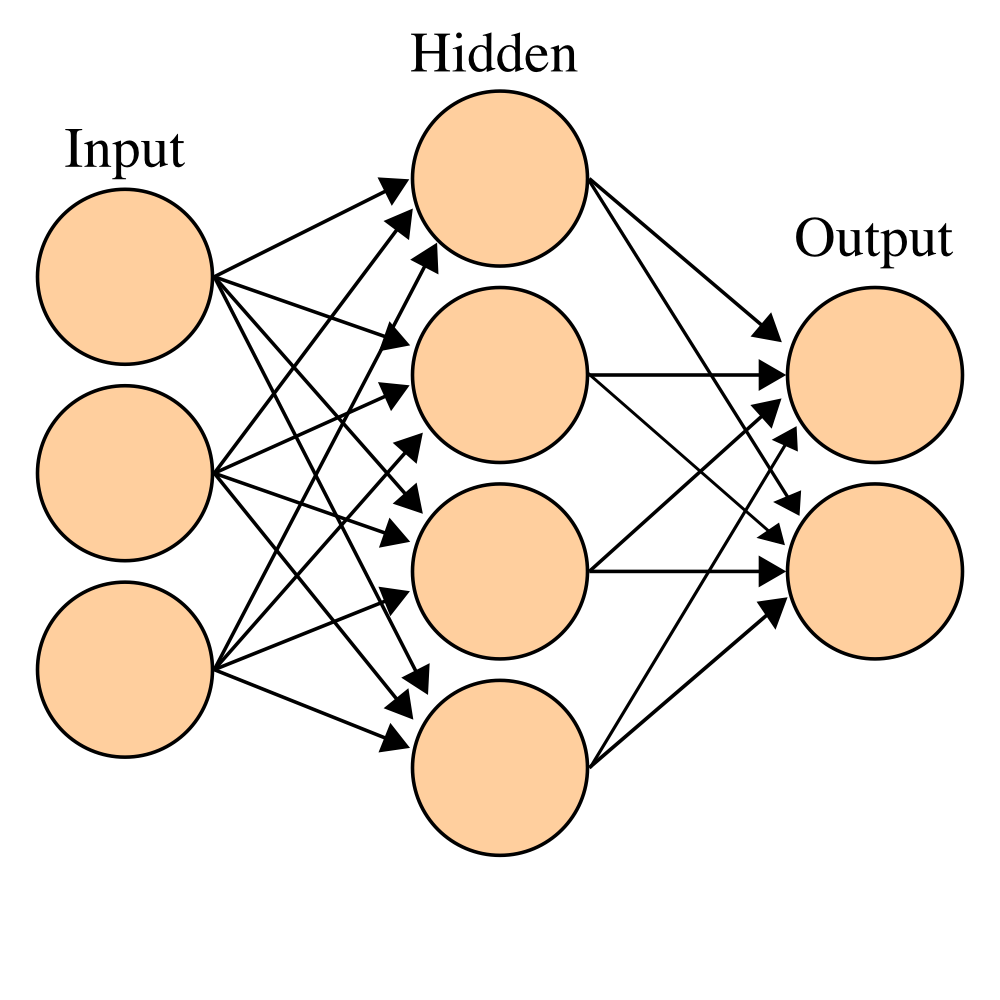
\includegraphics[scale=0.15]{Figures/ann.png}
    \caption{Example of ANN \cite{ann_wiki}}
    \label{fig:ann}
\end{figure}

\clearpage

\noindent Typically, a neural network is defined by three factors:
\begin{itemize}
    \item[1] How the different layers are interconnected
    \item[2] How the the weights are updated (learning process)
    \item[3] How the neuron's input value is converted to its output activation (activation function)
\end{itemize}



\section{Learning}
Lorem ipsum dolor sit amet, consectetur adipiscing elit, sed do eiusmod tempor incididunt ut labore et dolore magna aliqua. Ut enim ad minim veniam, quis nostrud exercitation ullamco laboris nisi ut aliquip ex ea commodo consequat. Duis aute irure dolor in reprehenderit in voluptate velit esse cillum dolore eu fugiat nulla pariatur. Excepteur sint occaecat cupidatat non proident, sunt in culpa qui officia deserunt mollit anim id est laborum. \\

\subsection{Supervised Learning}
Lorem ipsum dolor sit amet, consectetur adipiscing elit, sed do eiusmod tempor incididunt ut labore et dolore magna aliqua. Ut enim ad minim veniam, quis nostrud exercitation ullamco laboris nisi ut aliquip ex ea commodo consequat. Duis aute irure dolor in reprehenderit in voluptate velit esse cillum dolore eu fugiat nulla pariatur. Excepteur sint occaecat cupidatat non proident, sunt in culpa qui officia deserunt mollit anim id est laborum. \\

\subsection{Unsupervised Learning}
Lorem ipsum dolor sit amet, consectetur adipiscing elit, sed do eiusmod tempor incididunt ut labore et dolore magna aliqua. Ut enim ad minim veniam, quis nostrud exercitation ullamco laboris nisi ut aliquip ex ea commodo consequat. Duis aute irure dolor in reprehenderit in voluptate velit esse cillum dolore eu fugiat nulla pariatur. Excepteur sint occaecat cupidatat non proident, sunt in culpa qui officia deserunt mollit anim id est laborum. \\

\subsection{Reinforcement Learning}
Lorem ipsum dolor sit amet, consectetur adipiscing elit, sed do eiusmod tempor incididunt ut labore et dolore magna aliqua. Ut enim ad minim veniam, quis nostrud exercitation ullamco laboris nisi ut aliquip ex ea commodo consequat. Duis aute irure dolor in reprehenderit in voluptate velit esse cillum dolore eu fugiat nulla pariatur. Excepteur sint occaecat cupidatat non proident, sunt in culpa qui officia deserunt mollit anim id est laborum. \\

\section{Multilayer Perceptron}
Lorem ipsum dolor sit amet, consectetur adipiscing elit, sed do eiusmod tempor incididunt ut labore et dolore magna aliqua. Ut enim ad minim veniam, quis nostrud exercitation ullamco laboris nisi ut aliquip ex ea commodo consequat. Duis aute irure dolor in reprehenderit in voluptate velit esse cillum dolore eu fugiat nulla pariatur. Excepteur sint occaecat cupidatat non proident, sunt in culpa qui officia deserunt mollit anim id est laborum. \\

\subsection{Activation Function}
Lorem ipsum dolor sit amet, consectetur adipiscing elit, sed do eiusmod tempor incididunt ut labore et dolore magna aliqua. Ut enim ad minim veniam, quis nostrud exercitation ullamco laboris nisi ut aliquip ex ea commodo consequat. Duis aute irure dolor in reprehenderit in voluptate velit esse cillum dolore eu fugiat nulla pariatur. Excepteur sint occaecat cupidatat non proident, sunt in culpa qui officia deserunt mollit anim id est laborum. \\

\subsection{Layers}
Lorem ipsum dolor sit amet, consectetur adipiscing elit, sed do eiusmod tempor incididunt ut labore et dolore magna aliqua. Ut enim ad minim veniam, quis nostrud exercitation ullamco laboris nisi ut aliquip ex ea commodo consequat. Duis aute irure dolor in reprehenderit in voluptate velit esse cillum dolore eu fugiat nulla pariatur. Excepteur sint occaecat cupidatat non proident, sunt in culpa qui officia deserunt mollit anim id est laborum. \\

\subsection{Learning through Backpropagation}
Lorem ipsum dolor sit amet, consectetur adipiscing elit, sed do eiusmod tempor incididunt ut labore et dolore magna aliqua. Ut enim ad minim veniam, quis nostrud exercitation ullamco laboris nisi ut aliquip ex ea commodo consequat. Duis aute irure dolor in reprehenderit in voluptate velit esse cillum dolore eu fugiat nulla pariatur. Excepteur sint occaecat cupidatat non proident, sunt in culpa qui officia deserunt mollit anim id est laborum. \\

\subsubsection{Gradient Descent}
Lorem ipsum dolor sit amet, consectetur adipiscing elit, sed do eiusmod tempor incididunt ut labore et dolore magna aliqua. Ut enim ad minim veniam, quis nostrud exercitation ullamco laboris nisi ut aliquip ex ea commodo consequat. Duis aute irure dolor in reprehenderit in voluptate velit esse cillum dolore eu fugiat nulla pariatur. Excepteur sint occaecat cupidatat non proident, sunt in culpa qui officia deserunt mollit anim id est laborum. \\
